\documentclass[conference]{IEEEtran}
\IEEEoverridecommandlockouts
% The preceding line is only needed to identify funding in the first footnote. If that is unneeded, please comment it out.
\usepackage{cite}
\usepackage{amsmath,amssymb,amsfonts}
\usepackage{algorithmic}
\usepackage{graphicx}
\usepackage{textcomp}
\usepackage{xcolor}
\usepackage{booktabs}                        % AAB inserido
\usepackage[utf8]{inputenc}                  % AAB inserido
\usepackage{rotating}                        % AAB inserido
\ifCLASSOPTIONcompsoc                        % AAB inserido
\usepackage[caption=false,font=normalsize,labelfon
t=sf,textfont=sf]{subfig}
\else
\usepackage[caption=false,font=footnotesize]{subfi
g}
\fi
%\usepackage[round,sort,nonamebreak]{natbib}  % AAB inserido
%\usepackage[round,sort,nonamebreak]{natbib} % citação bibliográfica textual
\def\BibTeX{{\rm B\kern-.05em{\sc i\kern-.025em b}\kern-.08em
    T\kern-.1667em\lower.7ex\hbox{E}\kern-.125emX}}
%AAB
\DeclareMathOperator{\traco}{tr}
\graphicspath{{../Text/Dissertacao/figuras/}}
\begin{document}

\title{Fusão de evedência de bordas para canais de intensidade em imagens PolSAR\\
%{\footnotesize \textsuperscript{*}Note: Sub-titles are not captured in Xplore and should not be used}
\thanks{Bolsista Capes/PROSUP.}
}

\author{\IEEEauthorblockN{Anderson A. de Borba}
\IEEEauthorblockA{\textit{Dept. Engenharia Elétrica e Computação} \\
\textit{UPM - Universidade Presbiteriana Mackenzie}\\
IBMEC-SP\\
São Paulo, Brazil \\
anderson.borba@ibmec.edu.br}
\and
\IEEEauthorblockN{Maurício Marengoni}
\IEEEauthorblockA{\textit{Dept. Engenharia Elétrica e Computação} \\
\textit{UPM - Universidade Presbiteriana Mackenzie}\\
São Paulo, Brazil \\
mauricio.marengoni@mackenzie.br}
\and
\IEEEauthorblockN{\hspace{6cm} Alejandro C. Frery}
\IEEEauthorblockA{\textit{\hspace{6cm}Laboratório de Computação Científica e Análise Numérica - LACCAN} \\
\hspace{6cm}\textit{UFAL - Universidade Federal de Alagoas}\\
\hspace{6cm} Maceió, Brazil \\
\hspace{6cm}acfrery@gmail.com}
}

\maketitle

\begin{abstract}
Atualmente, na área de sensoriamento remoto, pode-de encontrar diferentes métodos para detecção e fusão de evidências de bordas. Entretanto, alguns desses  métodos, ao serem aplicados em imagens PolSAR, produzem resultados inadequados. Com intuito de melhorar sinal ruído, se tem investido em pesquisas com a utilização de modelagem estatística. O presente estudo, propõe um método de detecção e fusão de evidências bordas baseado no método da máxima verossimilhança, utilisando fusão de informações por média, SWT, PCA, e estatística ROC. Os precedimentos foram aplicados para os canais de intensidade de uma imagem real PolSAR. Os resultados indicam um bom desempenho do método na detecção de bordas com possíveis caminhos para pesquisas futuras .
\end{abstract}

\begin{IEEEkeywords}
PolSAR, detecção de bordas, Estimativa de máxima verossimilhança, Métodos de Fusão.
\end{IEEEkeywords}

\section{Introduction}\label{sec_01}
Neste trabalho será apresentado uma pesquisa sobre detecção e fusão de evidências de bordas, em imagens de radar de abertura sintética (\textit{Synthetic Aperture Radar} -- SAR) e nas imagens de radar polarimétrico de abertura sintética (\textit{Polarimetric Synthetic Aperture Radar} -- PolSAR), ambas requerem modelos e algoritmos adequados para o tratamento das suas características especiais.

Podemos citar diferentes técnicas de detecção de bordas, como no trabalho de \cite{slf_2008} onde é usado modelagem eletromagnética, ou os trabalhos de \cite{tlb, obw, flmc, fyf} os quais encontramos técnicas baseadas em métodos que estimam o gradiente. Assim como, no trabalho de \cite{bf}, são utilizadas técnicas baseadas nas cadeias de Markov. 

Em \cite{gfn} é descrita a comparação entre vários detectores de bordas que seguem a ideia deste trabalho. Técnicas baseadas nas modelagens estatísticas têm sido usadas na detecção de bordas em imagens SAR, podemos citar os trabalhos de \cite{gmbf, fbgm, horrit, gfn}. 

Atualmente as pesquisas em \textit{Deep Learning} têm sido largamente usadas na área de sensoriamento remoto, podemos encontrar aplicações nas referências \cite{bac, ztmxzxf, tabmm, xstz}. 

A área de fusão de imagens também é explorada neste trabalho. 
Um recente artigo, cujo autores são \cite{sglmla}, usa ideias do método \textit{random forest} aplicado em fusão de imagens PolSAR, adicionalmente, o artigo de \cite{sg} mostra outras técnicas de fusão de informação.  

O presente trabalho seguirá a abordagem de modelagem estatística, principalmente as técnicas descritas em \cite{fbgm, nhfc} usando a distribuição Wishart. Para realizar a fusão de informações temos como base as referências \cite{mit, sg}. 

O objetivo deste trabalho é detectar bordas em cada canal de uma imagem PolSAR e realizar a fusão das evidências de bordas, com a tarefa de entender a importância da informação de cada um desses canais. 

O artigo está estruturado da seguinte forma. A seção \ref{sec_02} é descrito a modelagem estatística para dados PolSAR, mostramos a modelagem usada nas seções \ref{sec_03}, \ref{sec_04} e \ref{sec_05}. Na seção \ref{sec_06} descrevemos os métodos de evidências de bordas com destaque ao método baseado em estatística ROC. Os resultdos numéricos estão descritos na seção \ref{sec_07} e finalmente na seção \ref{sec_08} serão apresentadas as conclusões do trabalho. 
\section{Modelagem estatística para dados PolSAR}\label{sec_02}
Os sistemas SAR, totalmente polarimétricos, transmitem pulsos de micro-ondas polarizados ortogonalmente e medem componentes ortogonais do sinal recebido. Para cada pixel temos uma matriz de coeficientes de espalhamento, que são números complexos e descrevem a transformação do campo eletromagnético transmitido para o campo eletromagnético recebido.

A transformação pode ser representada como
\begin{equation*}
 \left[
\begin{array}{c}
	E_{h}^{r}   \\
	E_{v}^{r}    \\
\end{array}
\right]
 = \frac{e^{\hat{\imath} kr}}{r}\left[
\begin{array}{cc}
	S_{hh}   & S_{hv}   \\
	S_{vh}   & S_{vv}   \\
\end{array}
\right]
 \left[
\begin{array}{c}
	E_{h}^{t}   \\
	E_{v}^{t}    \\
\end{array}
\right],
\end{equation*}
onde $k$ denota o número de onda, $\hat{\imath}$ é um número complexo e $r$ é a distância entre o radar e o alvo. O campo eletromagnético com componentes $E_{i}^{j}$ tem índice subscrito denotando a polarização horizontal ($h$) ou vertical ($v$),  enquanto o índice sobrescrito indica a onda recebida ($r$) ou transmitida ($t$). Definindo $S_{i,j}$ como os coeficientes de espalhamento complexo, tal que o índice $i$ e $j$ são associados com o recebimento e com a transmissão das ondas, por exemplo, o coeficiente de espalhamento $S_{hv}$ está associado a onda transmitida na direção vertical ($v$) e recebida na direção horizontal ($h$).

Sendo conhecido cada coeficiente, a matriz de espalhamento complexa $\mathbf{S}$ é definida por
\begin{equation}\label{eq_01}
\mathbf{S} = \left[
\begin{array}{cc}
	S_{hh}   & S_{hv}   \\
	S_{vh}   & S_{vv}   \\
\end{array}
\right],
\end{equation}
e se o meio de propagação das ondas é recíproco, então usaremos o teorema da reciprocidade \cite{lp} para definir a matriz de espalhamento como sendo hermitiana. Desta forma, a matriz de espalhamento pode ser representada pelo vetor
\begin{equation}\label{eq_02}
\mathbf{s} = \left[
\begin{array}{c}
	S_{hh}     \\
    S_{hv}     \\
	S_{vv}     \\
\end{array}
\right].
\end{equation}

E ainda, de acordo com as referências \cite{good} e \cite{lee} podemos considerar a hipótese da distribuição ser circular gaussiana multivariada complexa de média zero $N^C_3(0,\Sigma)$, cuja função densidade de probabilidade (pdf) é:
\begin{equation}\label{eq_03}
    f_{\mathbf{s}}(\mathbf{s};\mathbf{\Sigma})=\frac{1}{\pi^3|\mathbf{\Sigma}|} \exp(-\mathbf{s}^H\mathbf{\Sigma}^{-1}\mathbf{s}), \\
\end{equation}
onde $|\cdot|$ é a matriz determinante, o índice sobrescrito $H$ denota o número complexo conjugado e $\mathbf{\Sigma}$ é a matriz de covariância da amostra $\mathbf{s}$ tal que $\mathbf{\Sigma}=E(\mathbf{ss}^H)$. 

Por consequência da distribuição ser circular gaussiana multivariada complexa com média zero, e as entradas do vetor $\mathbf{s}$ são $\mathbf{s}_{ij}= R_{ij}+ i I_{ij}$, então por hipótese é exigido que $R_{ij}$ e $I_{ij}$ com $j=h,v$ satisfaçam 
\begin{itemize}
	\item[I-] $E[R_{ij}]=E[I_{ij}]=0,$
	\item[II-] $E[R_{ij}^2]=E[I_{ij}^2],$ 
	\item[II-] $E[R_{ij}I_{ij}]=0,$  
	\item[IV-] $E[R_{ij}R_{ij}]=E[I_{ij}I_{ij}],$ 
	\item[V-] $E[I_{ij}R_{ij}]=-E[R_{ij}I_{ij}].$
\end{itemize}
onde, $E[\cdot]$ denota o valor esperado. 

A modelagem estatistística descrita foi comprovada para dados SAR polarimétricos, confirmando-se que contém todas as informações necessárias para caracterizar o retroespalhamento, encontramos mais informações em \cite{sarabendi} e \cite{mfp}.
 
A modelagem estatística descrita, até aqui, trata apenas a modelagem de visada simples, porém, imagens polarimétricas são usualmente sujeitadas a um processo de múltiplas visadas, com o intuito de melhorar a razão entre o sinal e o seu ruído. Para esse fim, matrizes positivas definidas hermitianas estimadas são obtidas computando a média de $L$ visadas independentes de uma mesma cena. Resultando na matriz de covariância amostral estimada {\bf Z} conforme \cite{good, ade}
\begin{equation}\label{eq_04}
\begin{array}{ccc}
    \mathbf{Z}&=&\frac{1}{L}\displaystyle{\sum_{l=1}^{L} {\mathbf{s}_l}{\mathbf{s}_l}^H}, \\
\end{array}
\end{equation}
onde $\mathbf{s}_l$ com $l = 1, \dots, L$ amostras de $\mathit{L}$ vetores complexos distribuídos como $\mathbf{s}$, assim a matriz de covariância amostral associada a $\mathbf{s}_l$ denotam o espalhamento para cada visada $L$.

\section{Função de densidade Wishart múltiplas visadas}\label{sec_03}
O processo de múltiplas visadas tem a função densidade de probabilidade (pdf) Wishart  definida por,
\begin{equation}\label{eq_05}
    f_{\mathbf{Z}}(\mathbf{Z};\mathbf{\Sigma_{s}},L)=\frac{L^{mL}|\mathbf{Z}|^{L-m}}{|\mathbf{\Sigma_{s}}|^{L}\Gamma_m(L)} \exp(-L\traco(\mathbf{\Sigma_{s}}^{-1}\mathbf{Z})), \\
\end{equation} 
onde, $\traco(\cdot)$ é o operador traço de uma matriz, $\Gamma_m(L)$ é uma função Gamma multivariada definida por
\begin{equation*}
	\Gamma_m(L)=\pi^{\frac{1}{2}m(m-1)} \prod_{i=0}^{m-1}\Gamma(L-i) \\
\end{equation*}
e $\Gamma(\cdot)$ é a função Gamma e $m=3$ para o presente artigo. Podemos afirmar que $\mathbf{Z}$ é distribuído como uma distribuição Wishart denotando por $\mathbf{Z}\sim W(\mathbf{\Sigma_{s}}, L)$ e satisfazendo $E[\mathbf{Z}]=\mathbf{\Sigma_{s}}$. Sem perda de generalidade para o texto, vamos usar o símbolo $\mathbf{\Sigma}$ em detrimento a $\mathbf{\Sigma_{s}}$ para representar a matriz de covariância associada a $\mathbf{S}$.

\section{Deteção de Bordas}\label{sec_04}

Na literatura encontramos uma grande oferta de métodos clássicos para detectar bordas, por exemplo Sobel, Canny, Laplaciano da gaussiana(LoG) e LoG piramidal. Os métodos clássicos de detecção de bordas são construídos assumindo que o ruído é aditivo, o que torna esses métodos ineficientes para aplicação em imagens PolSAR.

Ao introduzir conceitos baseados nos artigos \cite{nhfc, gmbf} é possível propor um método de detecção de borda em imagens PolSAR com múltiplas visadas. A ideia principal é detectar o ponto de transição em uma faixa tão fina quanto possível entre duas regiões da imagem. O ponto de transição é definido como uma evidência de borda. Os ruídos nesse tipo de imagens são do tipo \textit{speckle}, os mesmos têm natureza multiplicativa, tornando a detecção de bordas em imagens SAR uma tarefa desafiadora.

As metodologias de detecção de bordas ocorrem em diversos estágios, abaixo enumeramos os estágios:
\begin{enumerate}
	\item identificar o centroide de uma região de interesse (ROI) de maneira automática, semiautomática ou manual;
	\item construir raios do centroide para fora da área de interesse;
	\item coletar dados em uma vizinhança em torno dos raios usando o algoritmo {\it Bresenham's midpoint line algorithm}, idealmente do tamanho de um pixel;
	\item detectar pontos na faixa de dados, os quais fornecem evidências de mudanças de propriedades estatísticas, ou seja, um ponto de transição que define uma evidência de borda;
	\item usar o método Simulated Anneling Generalizado (GenSA), referência \cite{xgsh}, para encontra pontos de máximo em funções de interesse;
	\item fusão de evidências de bordas detectadas nos canais $(hh)$, $(hv)$ e $vv$.
\end{enumerate}

\section{Método da máxima verosimilhança}\label{sec_05}

 A estimativa por máxima verossimilhança (MLE) é um método que, tendo um conjunto de dados e um modelo estatístico, estima os valores dos parâmetros do modelo maximizando uma função de probabilidade dos dados. O conceito de verossimilhança pode ser encontrado nos artigos \cite{nhfc, gmbf}.

Suponha $\mathbf{X}=(X_1,X_2,\dots,X_n)^T$ um vetor randômico distribuído de acordo com a função densidade de probabilidade (pdf) $f(\mathbf{x},\mathbf{\theta})$ com parâmetros $\mathbf{\theta}=(\theta_1,\dots,\theta_d)^T$ no espaço dos parâmetros $\Theta$. Definimos  a função de verossimilhança
\begin{equation*}
    L(\theta;\mathbf{X}) = \prod_{i=1}^{n}f(x_i;\theta), \\
\end{equation*}
e a função logarítmica de verossimilhança a qual podemos chamar de função de log-verossimilhança
\begin{equation}\label{eq_09}
	l(\theta;\mathbf{X})= \ln(L(\theta;\mathbf{X})) = \sum_{i=1}^{n}\ln(f(x_i;\theta)). \\
\end{equation}

De maneira simplificada a estimativa de máxima verossimilhança pode ser escrita por 
\begin{equation*}
    \widehat{\theta}= \text{arg}\,\max\limits_{\theta\in\Theta}L(\theta;\mathbf{x}),\\
\end{equation*}
e de maneira similar 
\begin{equation*}
    \widehat{\theta}= \text{arg}\,\max\limits_{\theta\in\Theta}l(\theta;\mathbf{x}).\\
\end{equation*}

Vamos usar o método de máxima verossimilhança aplicado na distribuição Wishart. Suponha $\mathbf{Z}=(\mathbf{Z}_1,\mathbf{Z}_2,\dots,\mathbf{Z}_N)^T$ um vetor randômico distribuído de acordo com a função densidade de probabilidade (pdf) (\ref{eq_05}) com parâmetros $\Sigma=\{\mathbf{\Sigma_A}, \mathbf{\Sigma_B\}}$ e $L$. Os parâmetros $\mathbf{\Sigma_A}$, $\mathbf{\Sigma_B}$ pertencem a duas amostras diferentes $A$ e $B$, nosso objetivo é detectar a fronteira entre as duas amostras.

A função de verossimilhança da amostra descrita por (\ref{eq_09}) é dada pela equação do produtório das funções de densidade, respectivamente associadas a cada amostra
\begin{equation}\label{eq_10}
	L(j)=\prod_{k=1}^{j}f_{\mathbf{Z}}(\mathbf{Z}_{k}^{'};\mathbf{\Sigma_{A}},L) \prod_{k=j+1}^{N}f_{\mathbf{Z}}(\mathbf{Z}_{k}^{'};\mathbf{\Sigma_{B}},L), \\
\end{equation}
onde $\mathbf{Z}_{k}^{'}$ é uma possível aproximação da matriz randômica descrita em (\ref{eq_04}).

Usando a equação (\ref{eq_09}), teremos a  função de log-verossimilhança.
\begin{equation}
\begin{array}{rcl}\label{eq_11}
	l(j)=\ln L(j)&=&\sum_{k=1}^{j}\ln f_{\mathbf{Z}}(\mathbf{Z}_{k}^{'};\mathbf{\Sigma_{A}},L)\\
	             &+&\sum_{k=j+1}^{N}\ln f_{\mathbf{Z}}(\mathbf{Z}_{k}^{'};\mathbf{\Sigma_{B}},L).
\end{array}
\end{equation}

Nesse momento, podemos realizar  manipulações algébricas na função densidade de probabilidade em cada termo do somatório e substituir nas duas parcelas da equação (\ref{eq_09}) resultando em
\begin{equation}
\begin{array}{lll}\label{eq_12}
	l(j)&=&N\left[mL\ln{\left(L\right)}-\ln{\left(\Gamma_m(L)\right)}\right]\\
	&-& L\left[j\ln{\left(|\mathbf{\Sigma_{A}}|\right)}+(N-j)\ln{\left(|\mathbf{\Sigma_{B}}|\right)}\right] \\
	&+&(L-m)\sum_{k=1}^{N}\ln{\left(|\mathbf{Z}_{k}^{'}|\right)}\\
	&-&L\left[\sum_{k=1}^{j}tr(\mathbf{\Sigma_{A}}^{-1}\mathbf{Z}_{k}^{'})+ \sum_{k=j+1}^{N}tr(\mathbf{\Sigma_{B}}^{-1}\mathbf{Z}_{k}^{'})\right]. \\
\end{array}
\end{equation}

A matriz $\Sigma$ pode ser encontrada usando o estimador de máxima verossimilhança denotado por $\widehat{\Sigma}$ de acordo com a referência \cite{good}. A equação (\ref{eq_13}) representa duas estimativas para a matriz de covariância $\Sigma$ que dependem da posição $j$
\begin{equation}\label{eq_13}
\widehat{\Sigma_{I}}(j) = \left\{
\begin{array}{lc}
	j^{-1}\sum_{k=1}^{j}\mathbf{Z}_{k}  & \mbox{se}\quad I=A,  \\
        (N-j)^{-1}\sum_{k=j+1}^{N}\mathbf{Z}_{k} & \mbox{se}\quad I=B. \\
\end{array}
\right.
\end{equation}

Na equação (\ref{eq_12}) podemos substituir a equação (\ref{eq_13}) e continuar a manipulação algébrica, tendo como resultado 
\begin{equation}\label{eq_14}
\begin{array}{rcl}
	l(j)&=&N\left[-mL(1-\ln{\left(L\right)})-\ln{\left(\Gamma_m(L)\right)}\right]\\
	&-&L\left[j\ln{\left(|\mathbf{\widehat{\Sigma}}_{A}(j)|\right)} +(N-j)\ln{\left(|\mathbf{\widehat{\Sigma}}_{B}(j)|\right)}\right]\\
	&+&(L-m)\sum_{k=1}^{N}\ln{\left(|\mathbf{Z}_{k}^{'}|\right)}. \\
\end{array}
\end{equation}

O argumento máximo  $\widehat{\jmath}_{ML}$ é uma evidência de borda que será usada nos métodos de fusão.
\begin{equation*}
\begin{array}{rcl}
	\widehat{\jmath}_{ML}&=&\text{arg}\max\limits_{j}l(j).  \\
\end{array}
\end{equation*}
\section{Métodos de fusão de evidências de bordas}\label{sec_06}
\subsection{Média simples}
O método de fusão com média simples propõe a média aritmética das evidências de bordas, em cada canal. A fusão das evidências de bordas pode ser calculada por
\begin{equation}
	IF(x,y)=\frac{1}{nc}\sum_{i=1}^{nc}IE_i(x,y),
\end{equation}
onde $nc$ é o número de canais a serem utilizados na fusão. Podemos obter mais detalhes na referência \cite{mit}.
\subsection{Transformada wavelet estacinária - SWT} Esta seção, novamente é baseada na referência \cite{n_r}. O método de fusão SWT pode ser descrito pelos seguintes passos:
\begin{itemize}
\item[-] calcule a decomposição SWT obtendo $L_{HH}$, $L_{HL}$, $L_{LH}$ e $L_{LL}$ para cada canal;
\item[-] nas decomposições $L_{HH}$ é realizada a média aritmética de todos canais, pixel a pixel, e nas decomposições $L_{HL}$, $L_{LH}$ e $L_{LL}$, é encontrado o máximo entre cada canal, pixel a pixel, restando uma nova decomposição $\bar{L}_{HH}$, $\bar{L}_{HL}$, $\bar{L}_{LH}$ e $\bar{L}_{LL}$;
\item[-] realizando a transformação inversa de SWT, obtemos a imagem com a fusão das evidências de bordas $IF(x,y)$.  
\end{itemize}
\subsection{Pincipal component analysis - (PCA) }
Esta seção é baseada na referência \cite{n_r} e \cite{mit}. O método de fusão baseado no PCA pode ser descrito pelos seguintes passos:
\begin{itemize}
\item[-] organizar os dados de forma a ter cada imagem em um vetor coluna, formando uma matriz $Y$ de dimensão $l\times nc$, onde $l=m\cdot n$, representa a multiplicação das $m$ linhas e $n$ colunas das matrizes a serem utilizadas na fusão;
\item[-] calcule a média dos elementos dessas colunas, gerando um vetor de dimensão $1\times nc$;
\item[-] subtrair a média de cada coluna da matriz $Y$. Resultando em uma matriz $X$ de mesma dimensão de $Y$; 
\item[-] ache a matriz de covariância $C$ proveniente de $X$, calculando $C=XX^T$;
\item[-] calcule os autovalores $\Lambda$ e os autovetores $D$, e ordene os autovalores e autovetores em ordem decrescente. As matrizes geradas pelos autovalores, na diagonal principal, e os autovetores colocados em coluna, têm dimensões $nc\times nc$;
\item[-] compute as componentes $P_i=\frac{V_i}{\sum_{i=1}^l V_i}$ com $i=1,\dots,nc$;
\item[-] realizamos a fusão $IF(x,y)=\sum_{i=1}^{nc}P_iIE_i(x,y)$. Lembrando que o $\sum_{i=1}^{nc}P_i=1$.
\end{itemize}

\subsection{Estatística ROC}
O método Estatística ROC foi proposto e descrito em detalhes nas referências \cite{gs} e \cite{fawcett}. O método descreve um modelo estatístico para obter informações de maneira automática, de diversas imagens, ou, em diversos canais. Podemos descrever o método no seguinte procedimento:
\begin{itemize}
\item[-] obter as evidências de bordas nos canais, aplicando o método descrito nesse artigo. Armazene essas evidências de bordas em matrizes $E_i$, com $i=1,\cdots,nc$ de maneira binária;
\item[-] defina uma matriz de frequência de bordas $V$. A matriz  $V$ é gerada, somando as evidências de bordas $E_i$;
\item[-] utilize limiares variando de $t=1,\dots,nc$ gerando matrizes $M_t$;
\item[-] faça a comparação de cada $M_t$, fixada com todas as $E_i$,  encontre a matriz de confusão para gerar a curva ROC. O ponto da curva ROC que se aproximar (no sentido da distância euclidiana) da linha diagnóstico, terá seu limiar considerado ótimo;
\item[-] a matriz $M_t$, que corresponde ao limiar mais próximo da linha diagnóstico, é a fusão de evidências de bordas.
\end{itemize}
  
\section{Resultados numéricos}\label{sec_07}

A imagem PolSAR, com 4 visadas da região de Flevoland na Holanda, foi usada para os testes numéricos. A figura (\ref{fig_01}) mostra a região de interesse, onde construímos as retas radiais para a detecção de bordas.

 A detecção de bordas e suas posteriores fusão de evidências foram realizadas nessa região de interesse, com intuito de entender a ponderação de cada canal, na formação da imagem.

Neste trabalho a detecção de bordas foi realizada nos canais de intensidade (hh), (hv) e (vv), e posteriormente, usadas para a fusão de informações.   
%\begin{figure}[hbt]
%\centering
%	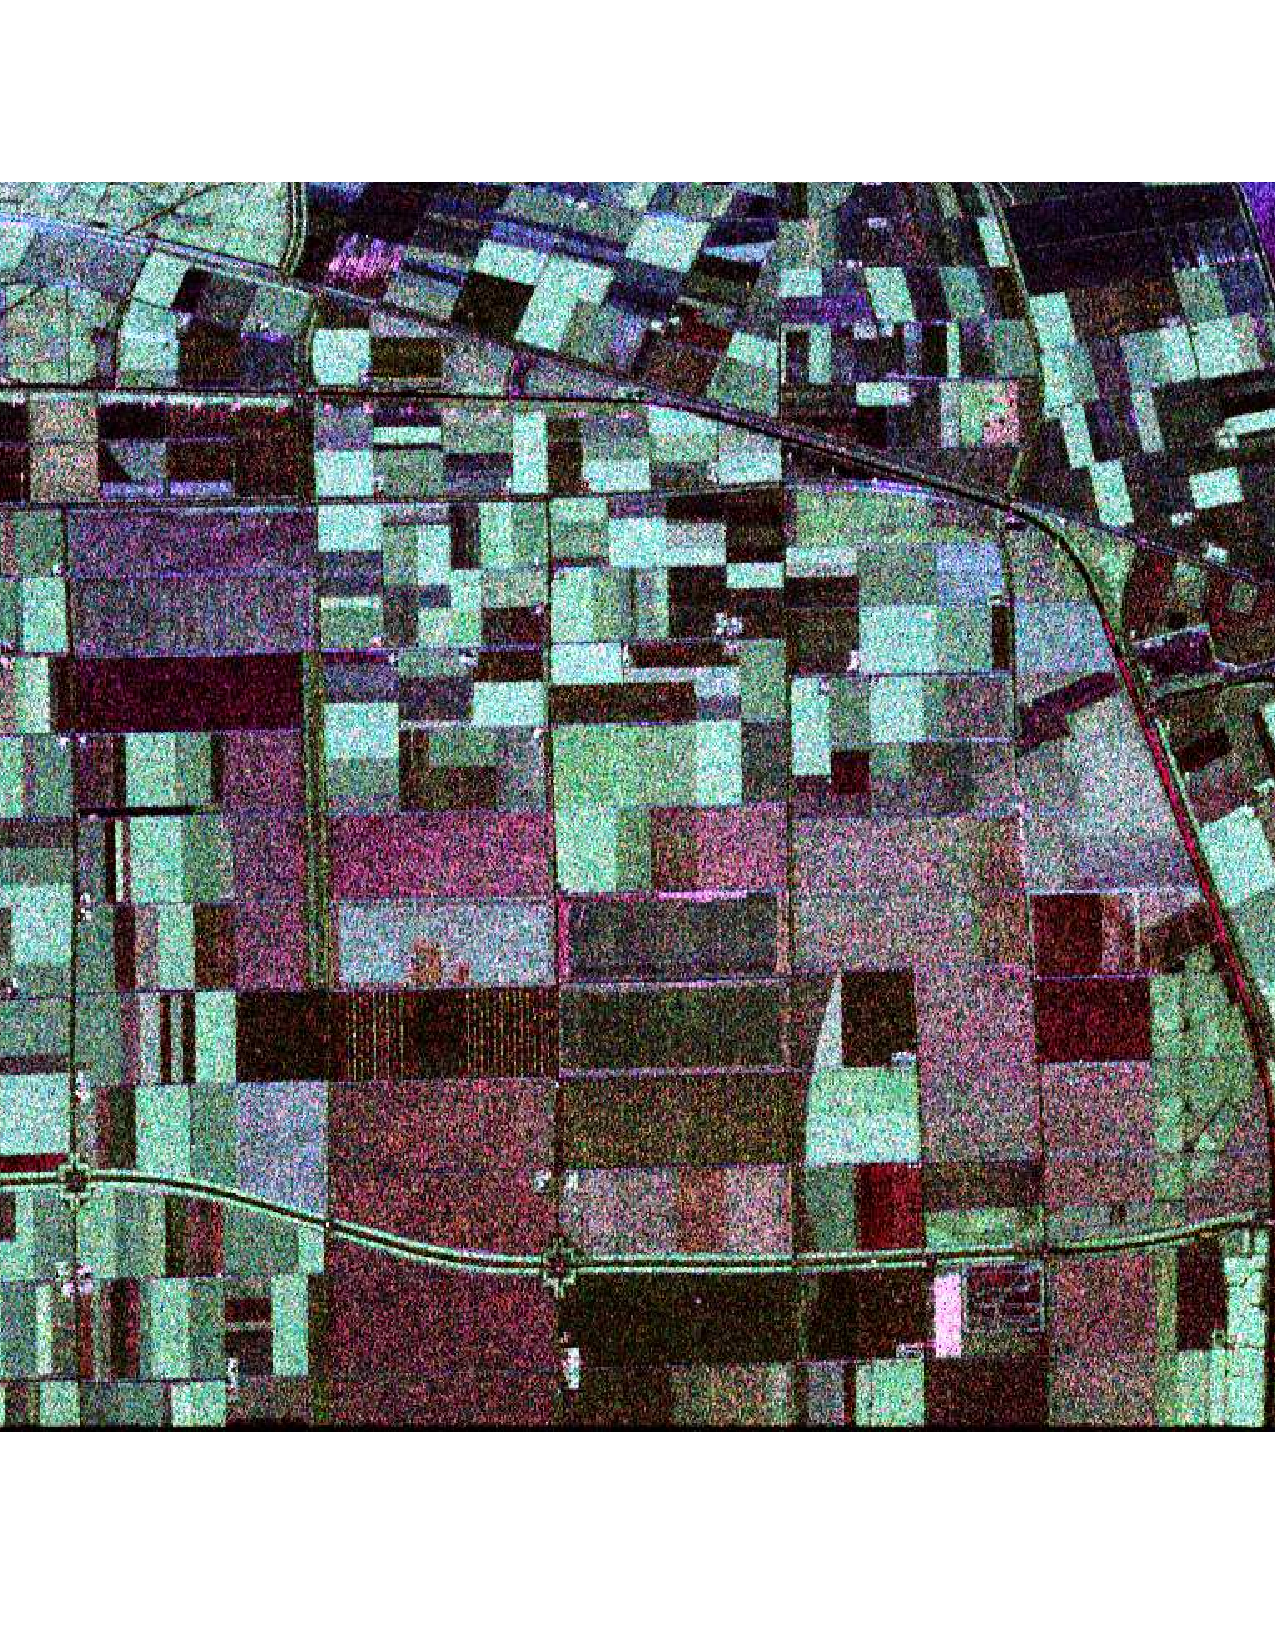
\includegraphics[scale=0.3]{flevoland_4_look.pdf}
%	\vspace{-1.0cm}
%		\caption{Imagem de Flevoland com 4 visadas.}
%\label{cap_acf_fig10}
%\end{figure}
\begin{figure}[hbt]
\centering
	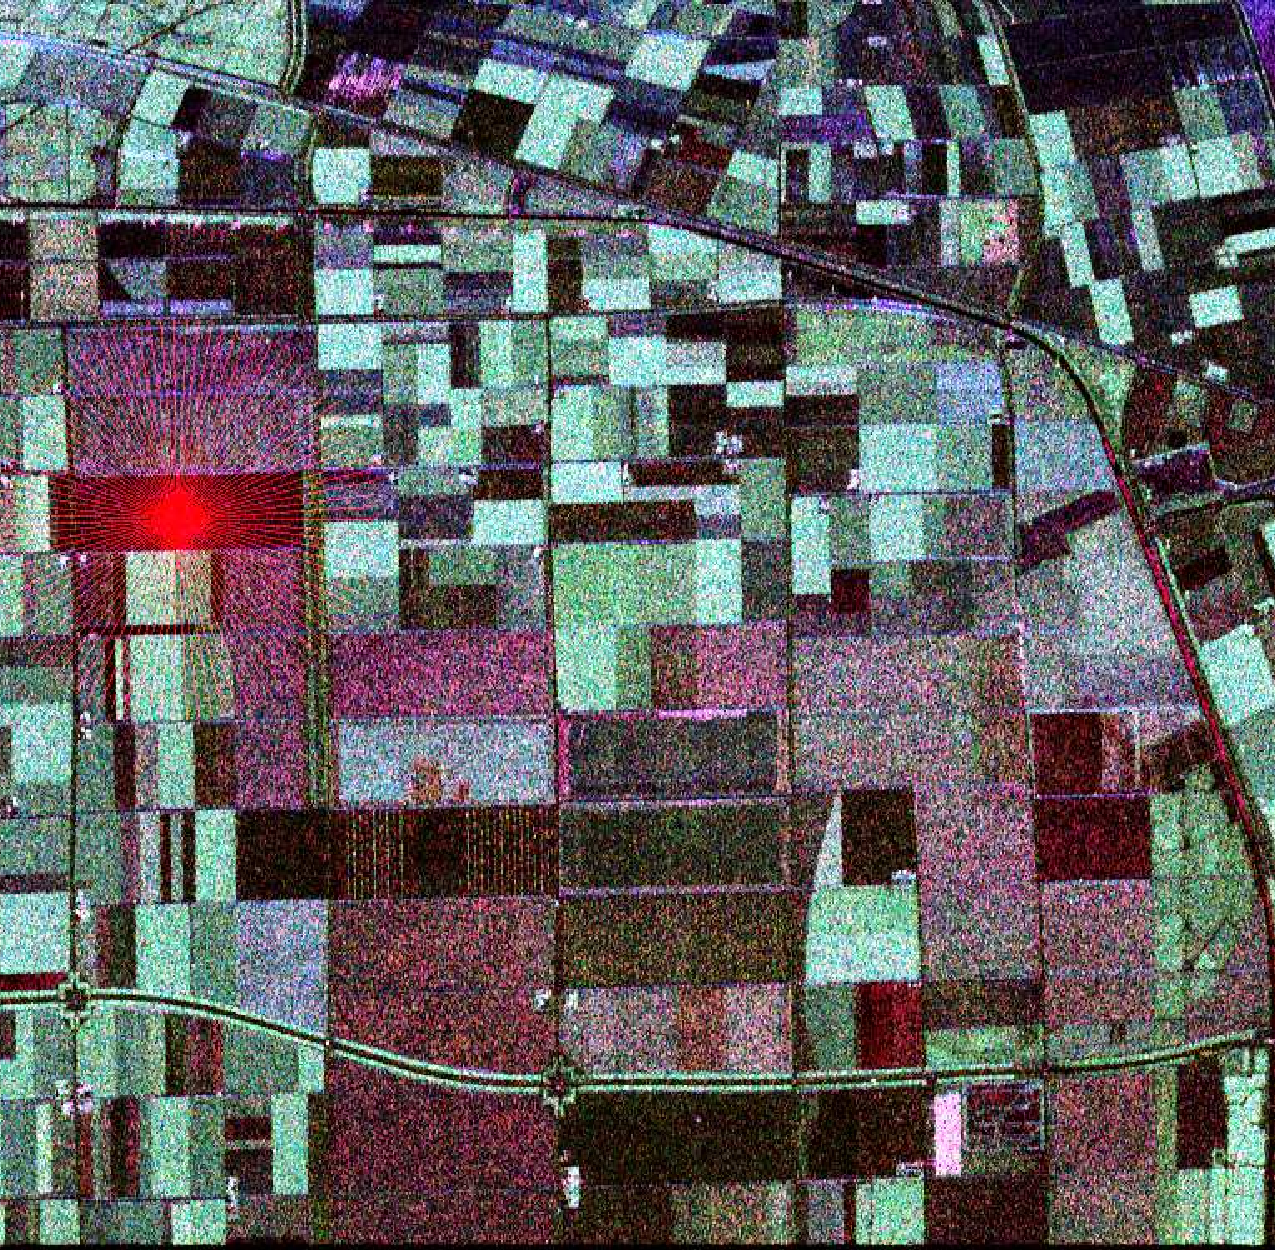
\includegraphics[scale=0.3]{flevoland_radial_4_look.pdf}
			\vspace{-1.0cm}
	\caption{Região de interesse (ROI) na imagem de Flavoland.}
\label{fig_01}
\end{figure}

As figuras (\ref{fig_02}), (\ref{fig_03}) e (\ref{fig_04}) mostram, respectivamente, os algoritmos de detecção das evidência de bordas, aplicados nos canais (hh), (hv) e (vv). 

O algoritmo para detectar as evidências de bordas funcionou bem nos canais (hh) e (hv), atingindo uma melhor acurácia em relação ao canal (vv).  

No canal (vv) foi detectado bordas que não fazem parte da região homogênea de interesse, porém, fazem parte de outras bordas da imagem, pesquisando o motivo desse fato, foi analisado a função $l(j)$ e constatado que a função apresenta dois picos, representando possíveis evidências de bordas, no qual o maior foi detectado corretamente. 
\begin{figure}[hbt]
	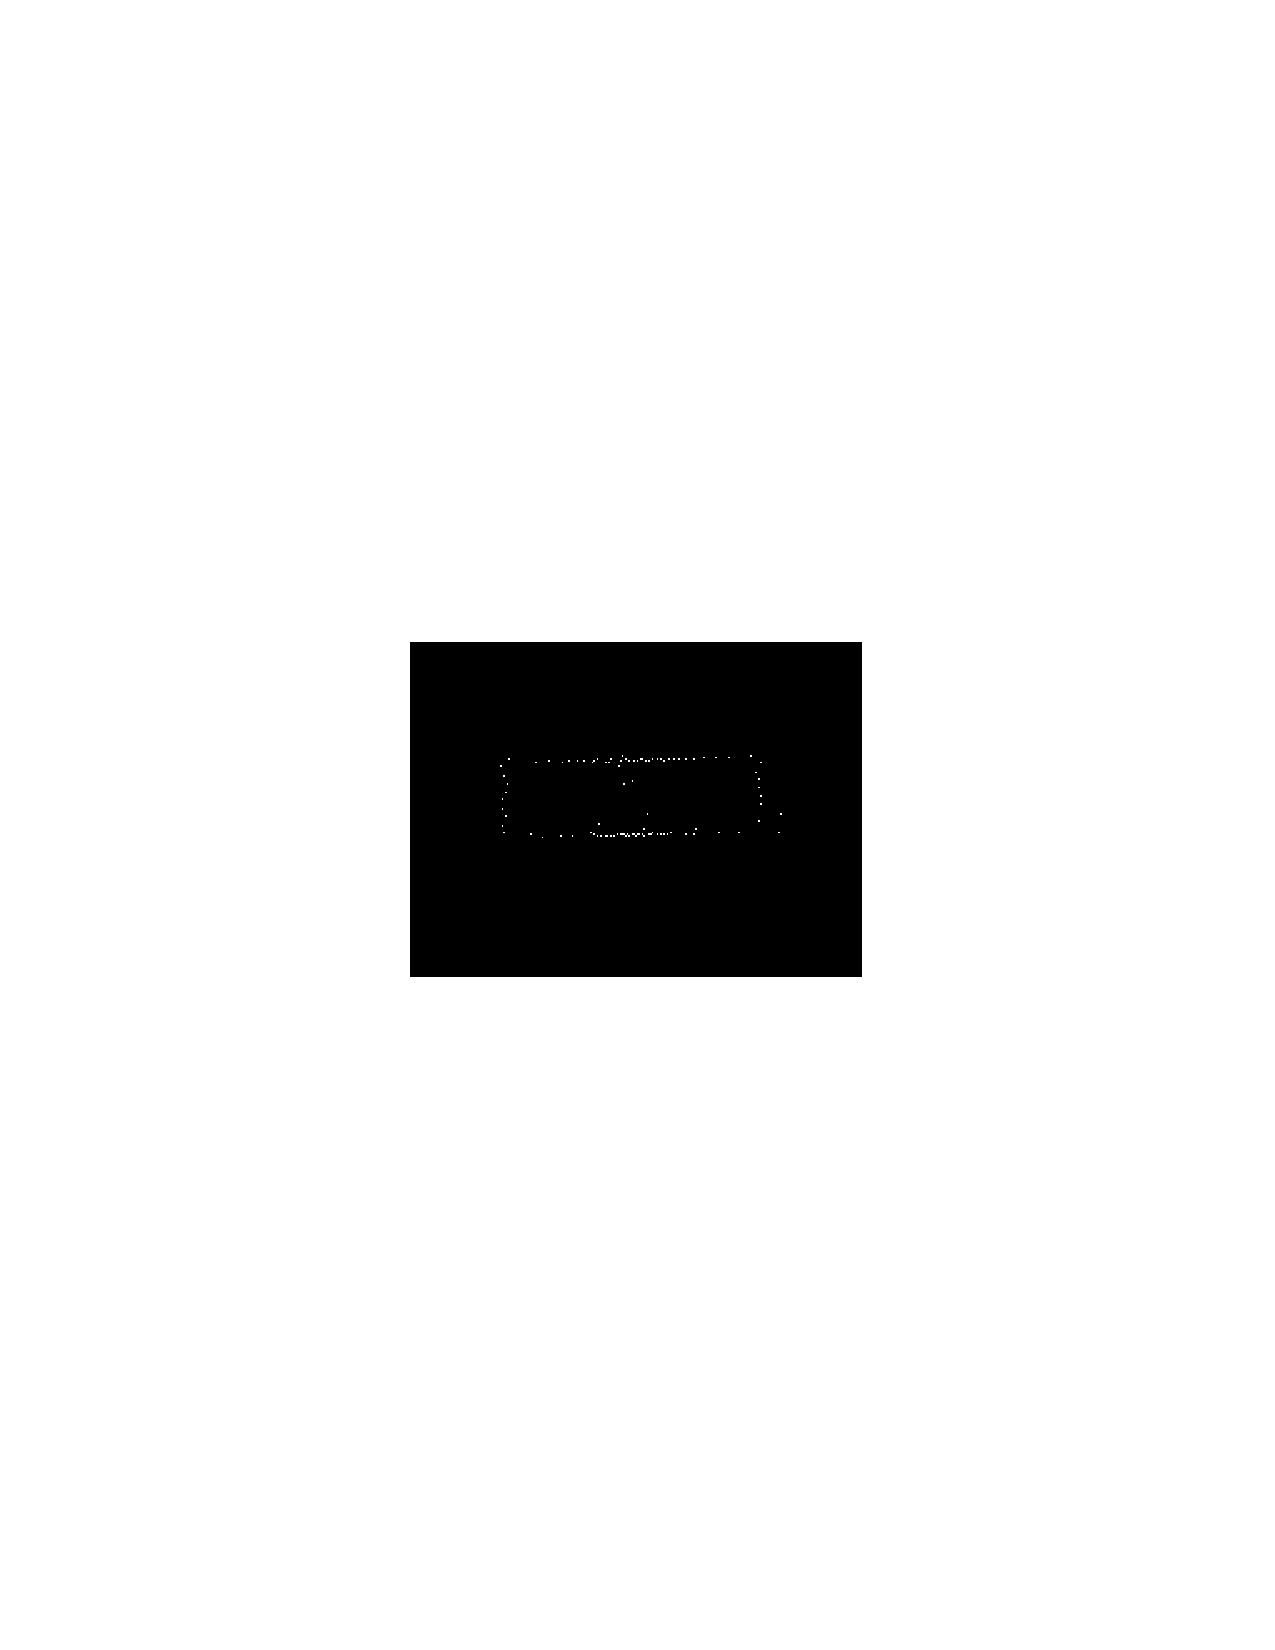
\includegraphics[scale=0.75]{flevoland_hh_evid_crop.pdf}
		\vspace{-6.0cm}
	\caption{Evidências de bordas detectadas no canal (hh).}
\label{fig_02}
\end{figure}
\begin{figure}[hbt]
	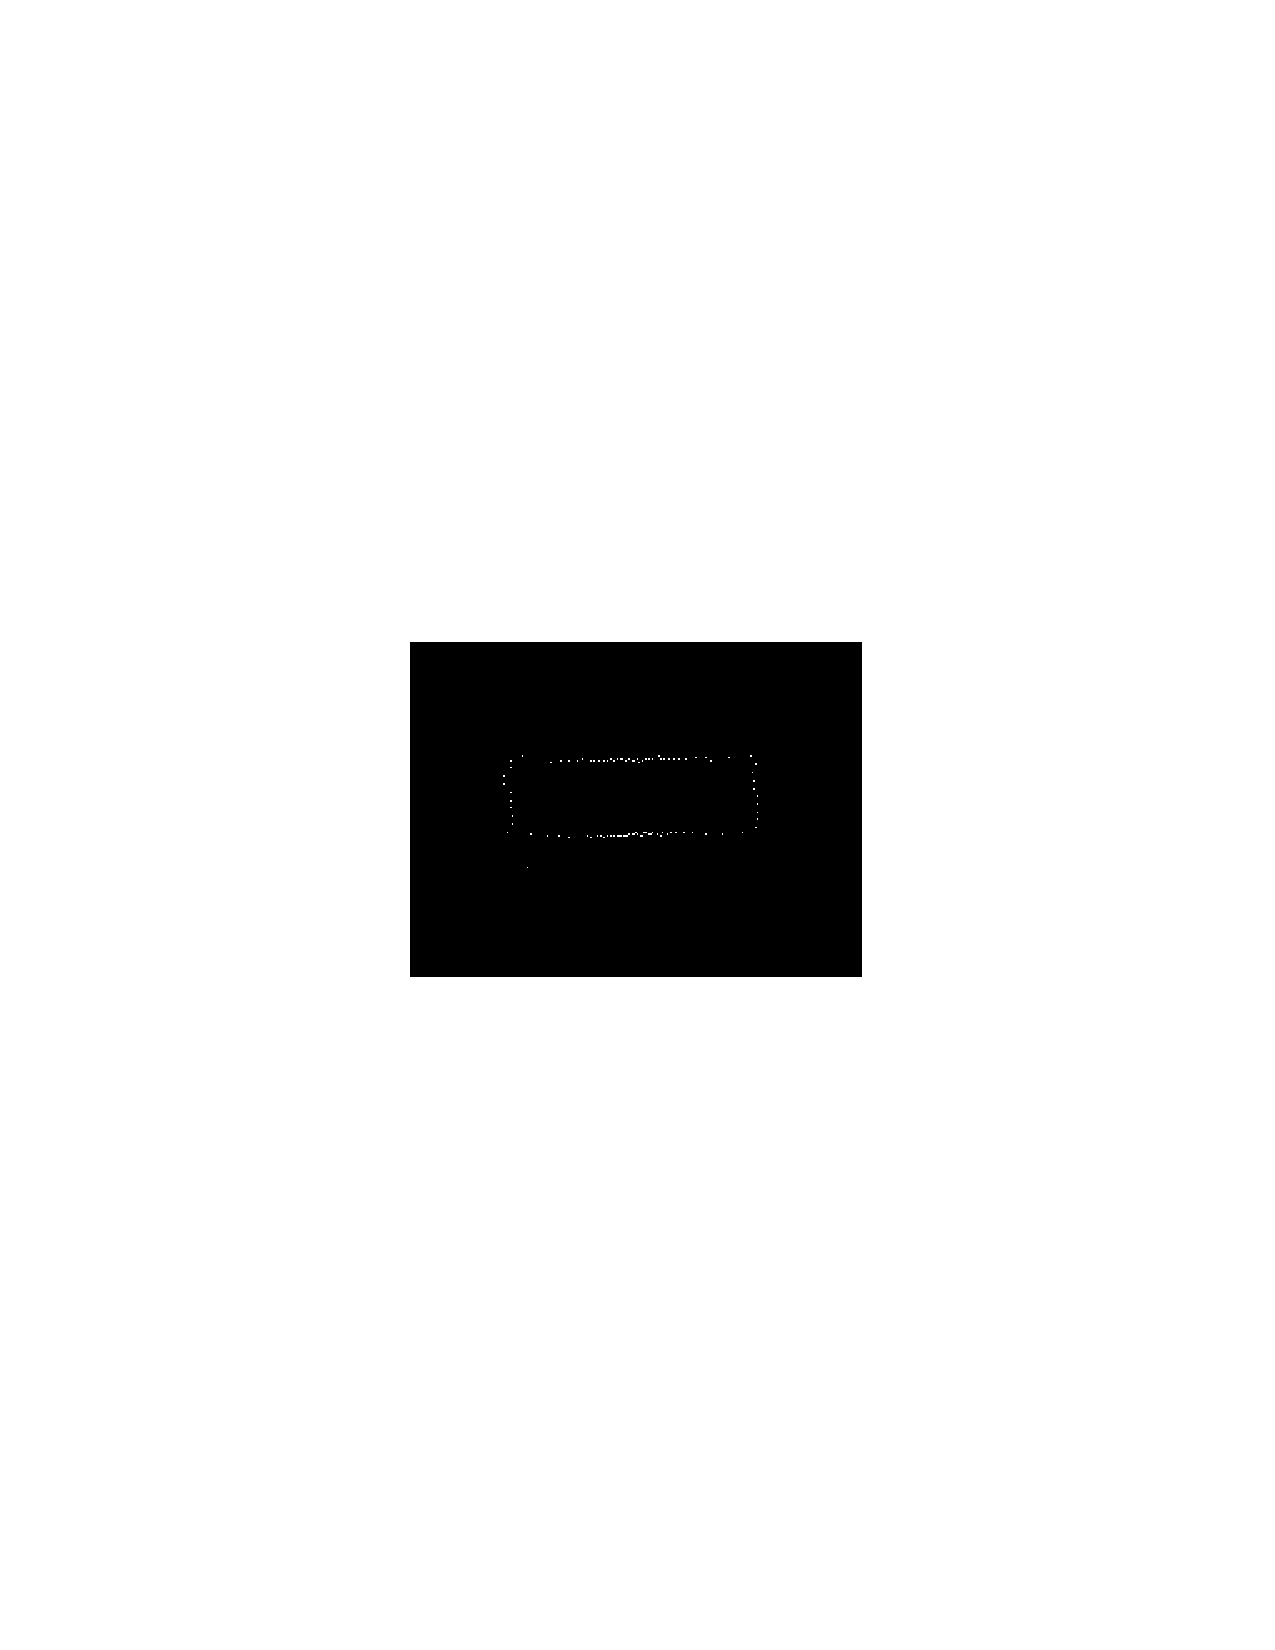
\includegraphics[scale=0.75]{flevoland_hv_evid_crop.pdf}
	\vspace{-6.0cm}
	\caption{Evidências de bordas detectadas no canal (hv).}	
\label{fig_03}
\end{figure}
\begin{figure}[hbt]
	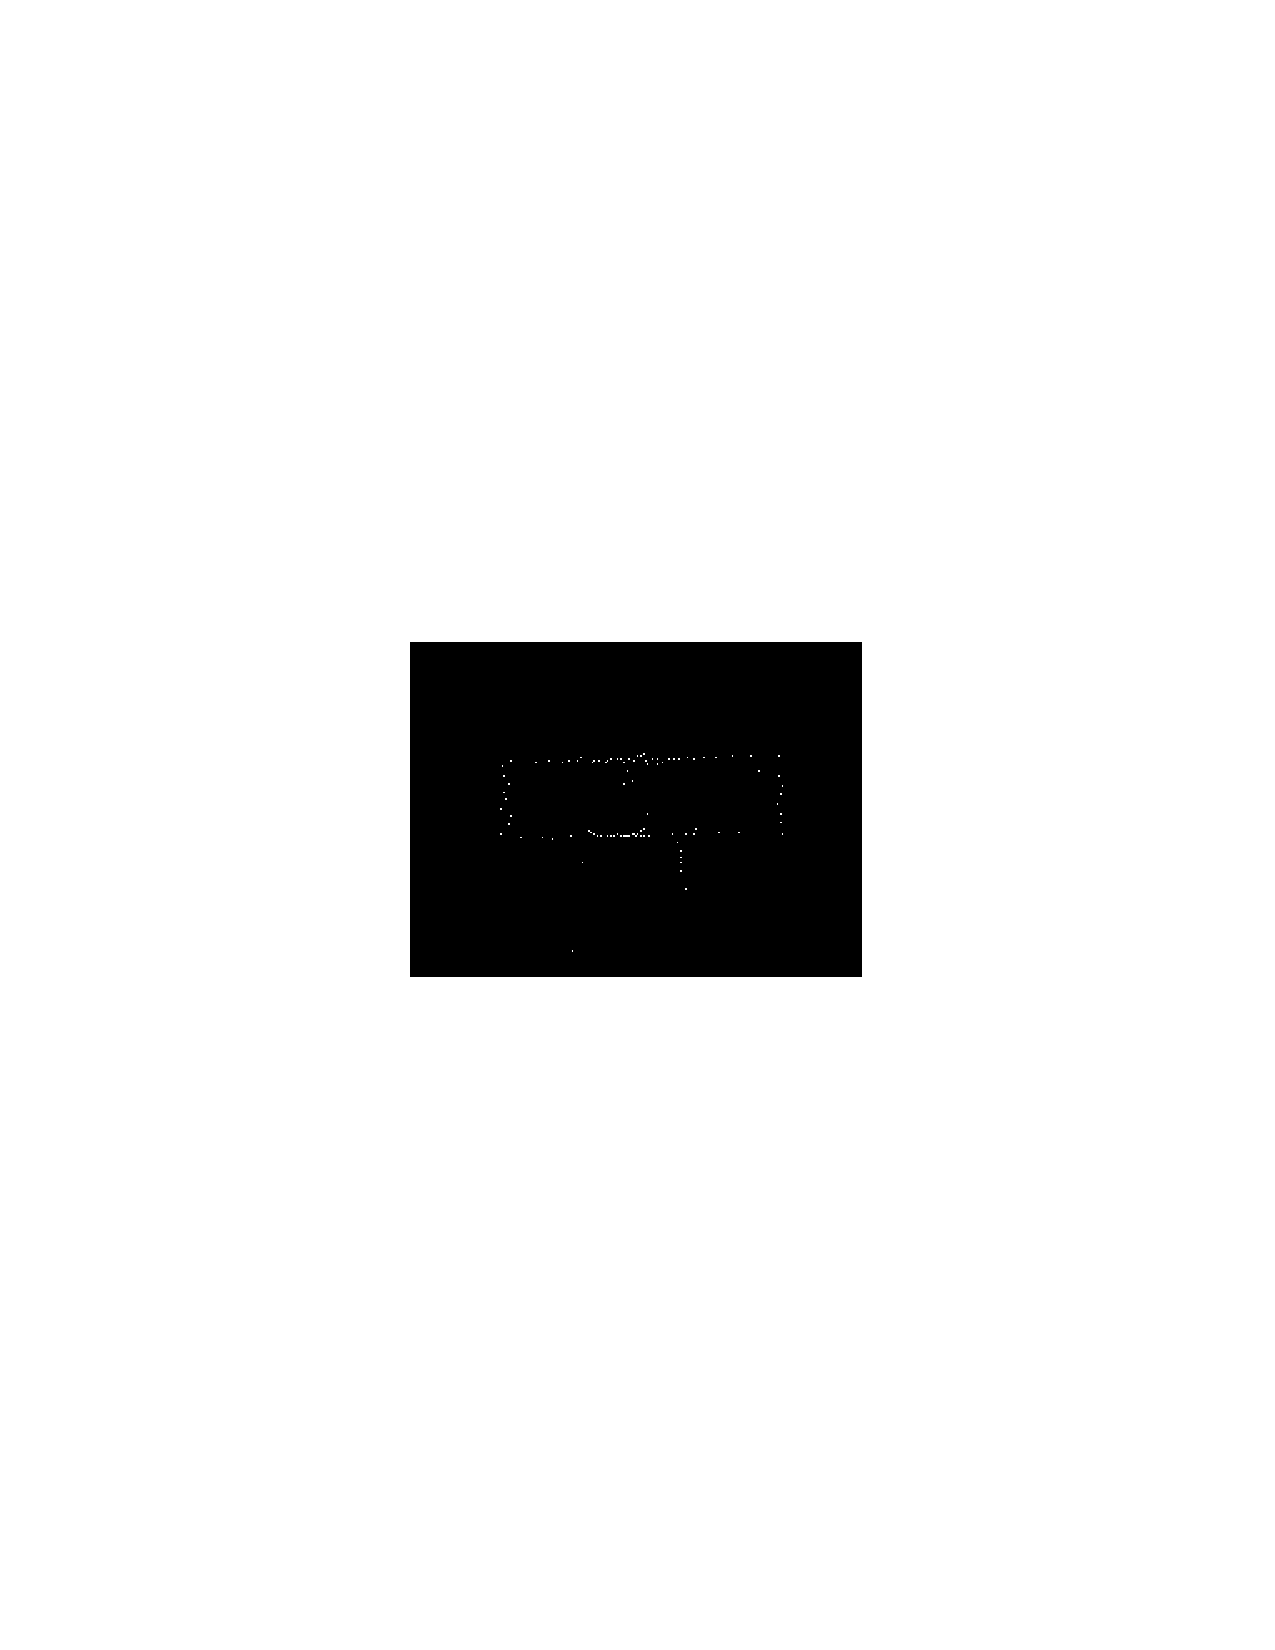
\includegraphics[scale=0.75]{flevoland_vv_evid_crop.pdf}
	\vspace{-6.0cm}
	\caption{Evidências de bordas detectadas no canal (vv).}
\label{fig_04}
\end{figure}

As figuras (\ref{fig_05}) até (\ref{fig_08}) mostram, respectivamente, a fusão de evidências para os métodos descritos neste artigo. Em ordem, listamos o método que mostra a média de evidências de bordas, o método que usa a Stationary wavelet transform (SWT), o método que usa a Principal component analysis (PCA) e finalmente, o método baseado na estatística ROC.

Os métodos mostrados nas figuras (\ref{fig_05}), (\ref{fig_06}) e (\ref{fig_07}) usam todos os pixeis detectados nos diferentes canais. Cada método pondera os pixeis nos diferentes canais com suas características. A média pondera, igualmente, os pixeis. O (SWT) encontra os coeficientes da combinação linear das suas bases de wavelets, e o (PCA) pondera os autovetores da matriz de covariância.

O método da estatística ROC não usa todos os pixeis dos canais, pois o método é baseado em limiares descartando pixeis. Isso se observou na na figura (\ref{fig_08}).
\begin{figure}[hbt]
	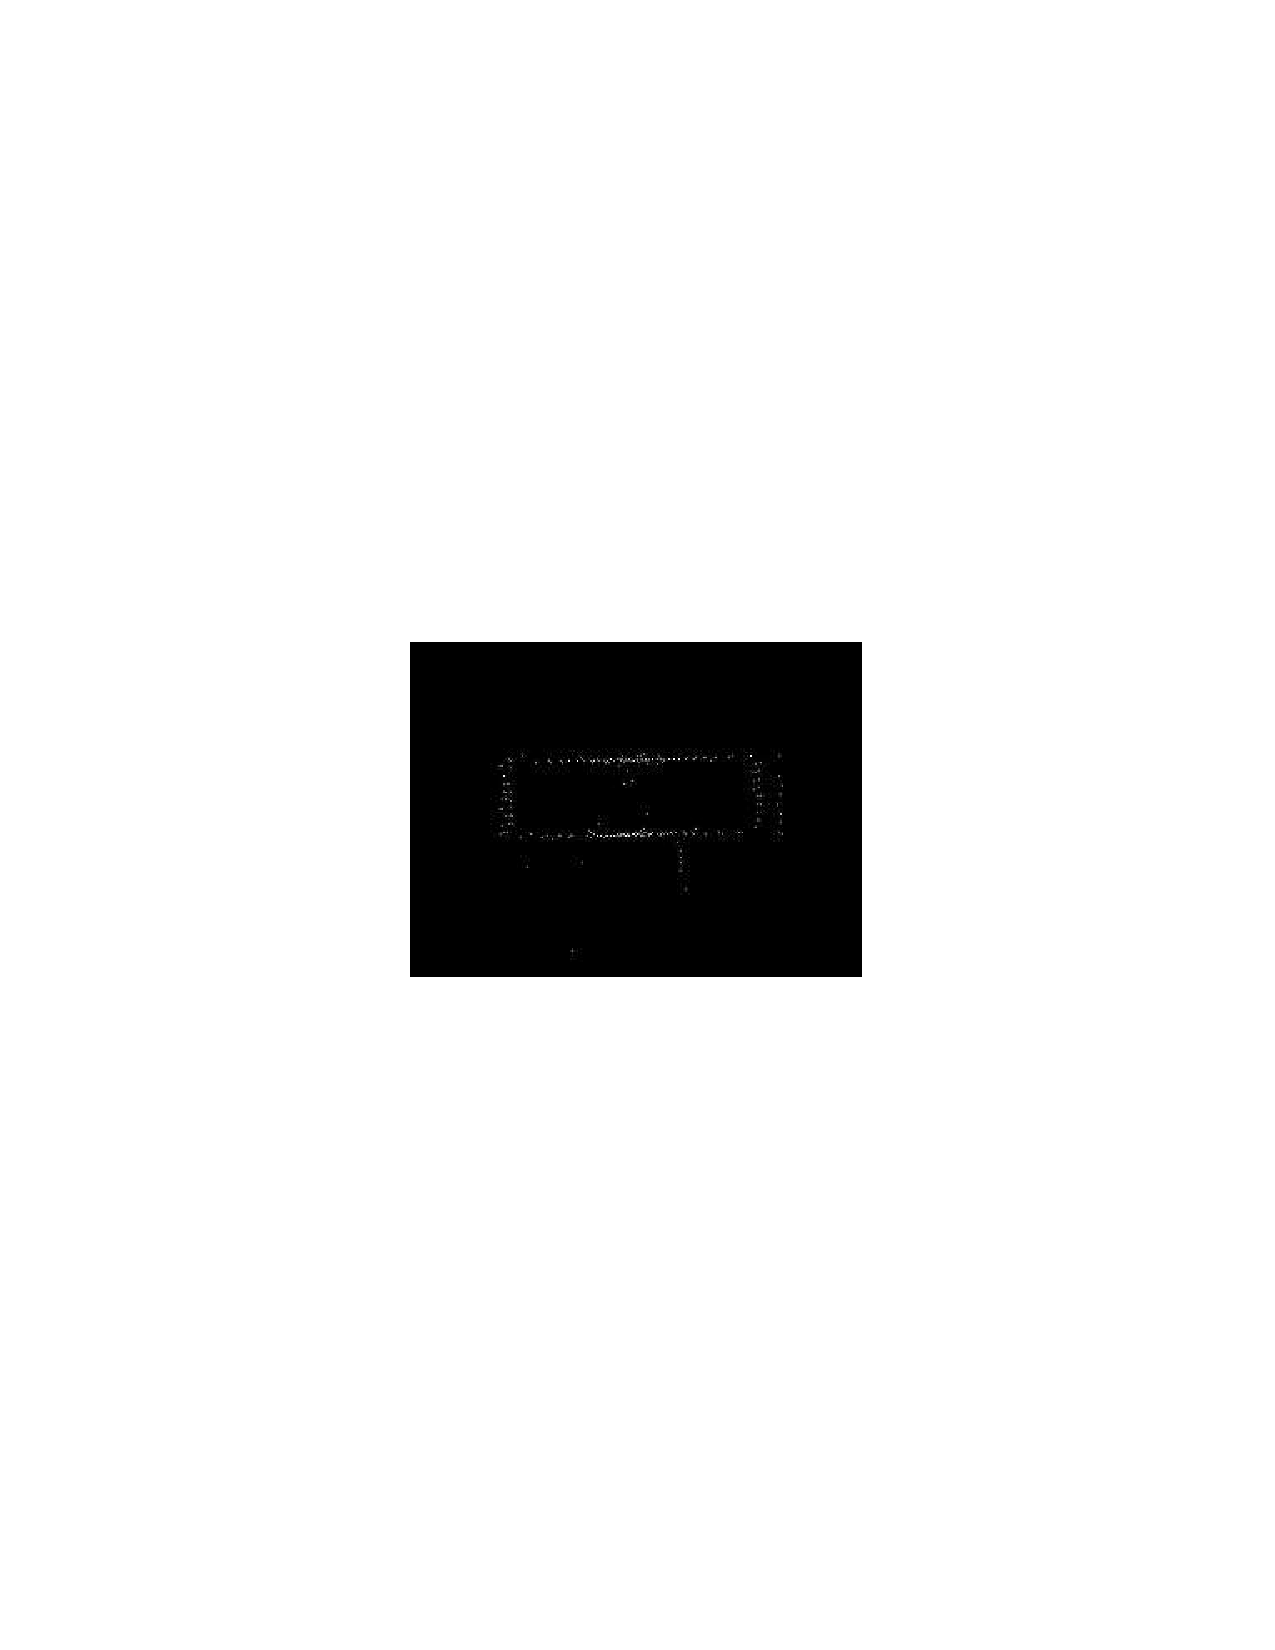
\includegraphics[scale=0.5]{flevoland_fusao_swt_crop.pdf}
	\caption{Fusão de evidências de bordas usando o método da média.}
\label{fig_05}
\end{figure}
\begin{figure}[hbt]
	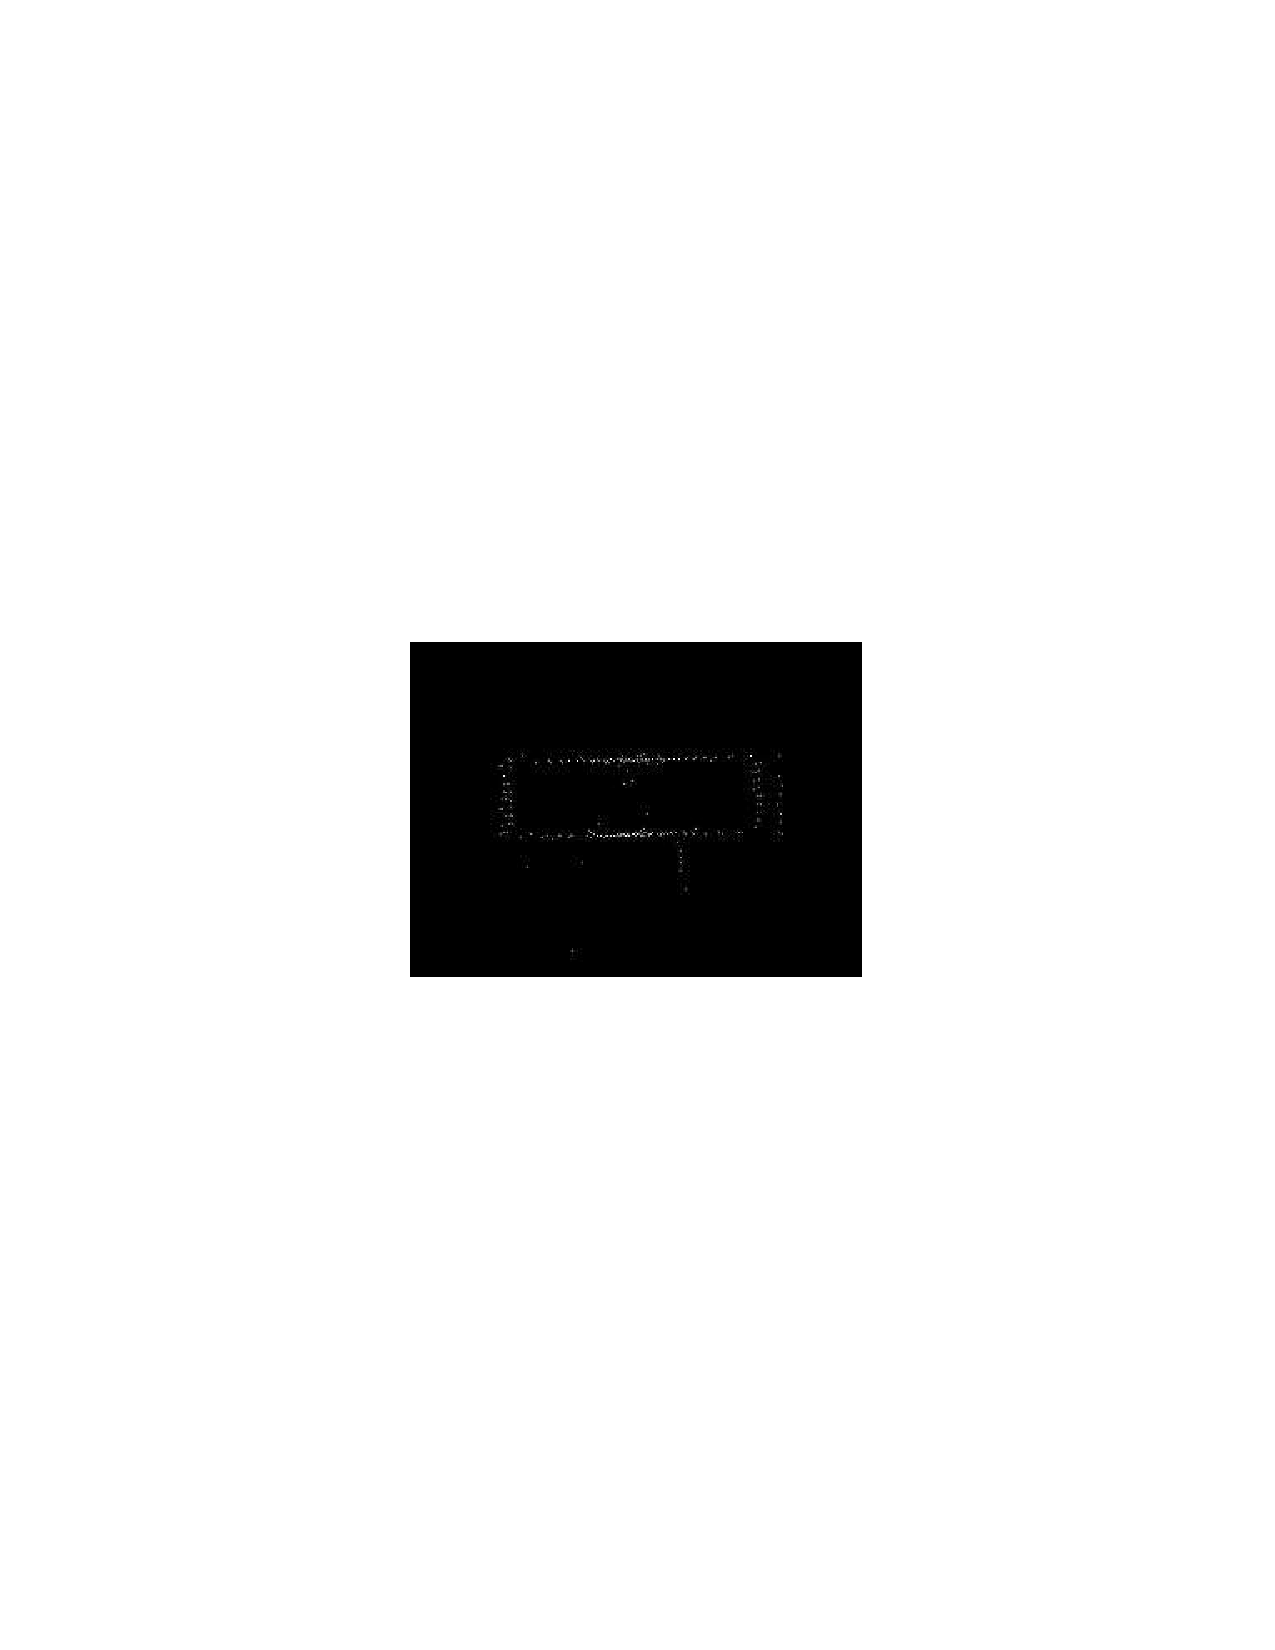
\includegraphics[scale=0.5]{flevoland_fusao_swt_crop.pdf}
	\caption{Fusão de evidências de bordas usando o método swt.}
\label{fig_06}
\end{figure}
\begin{figure}[hbt]
	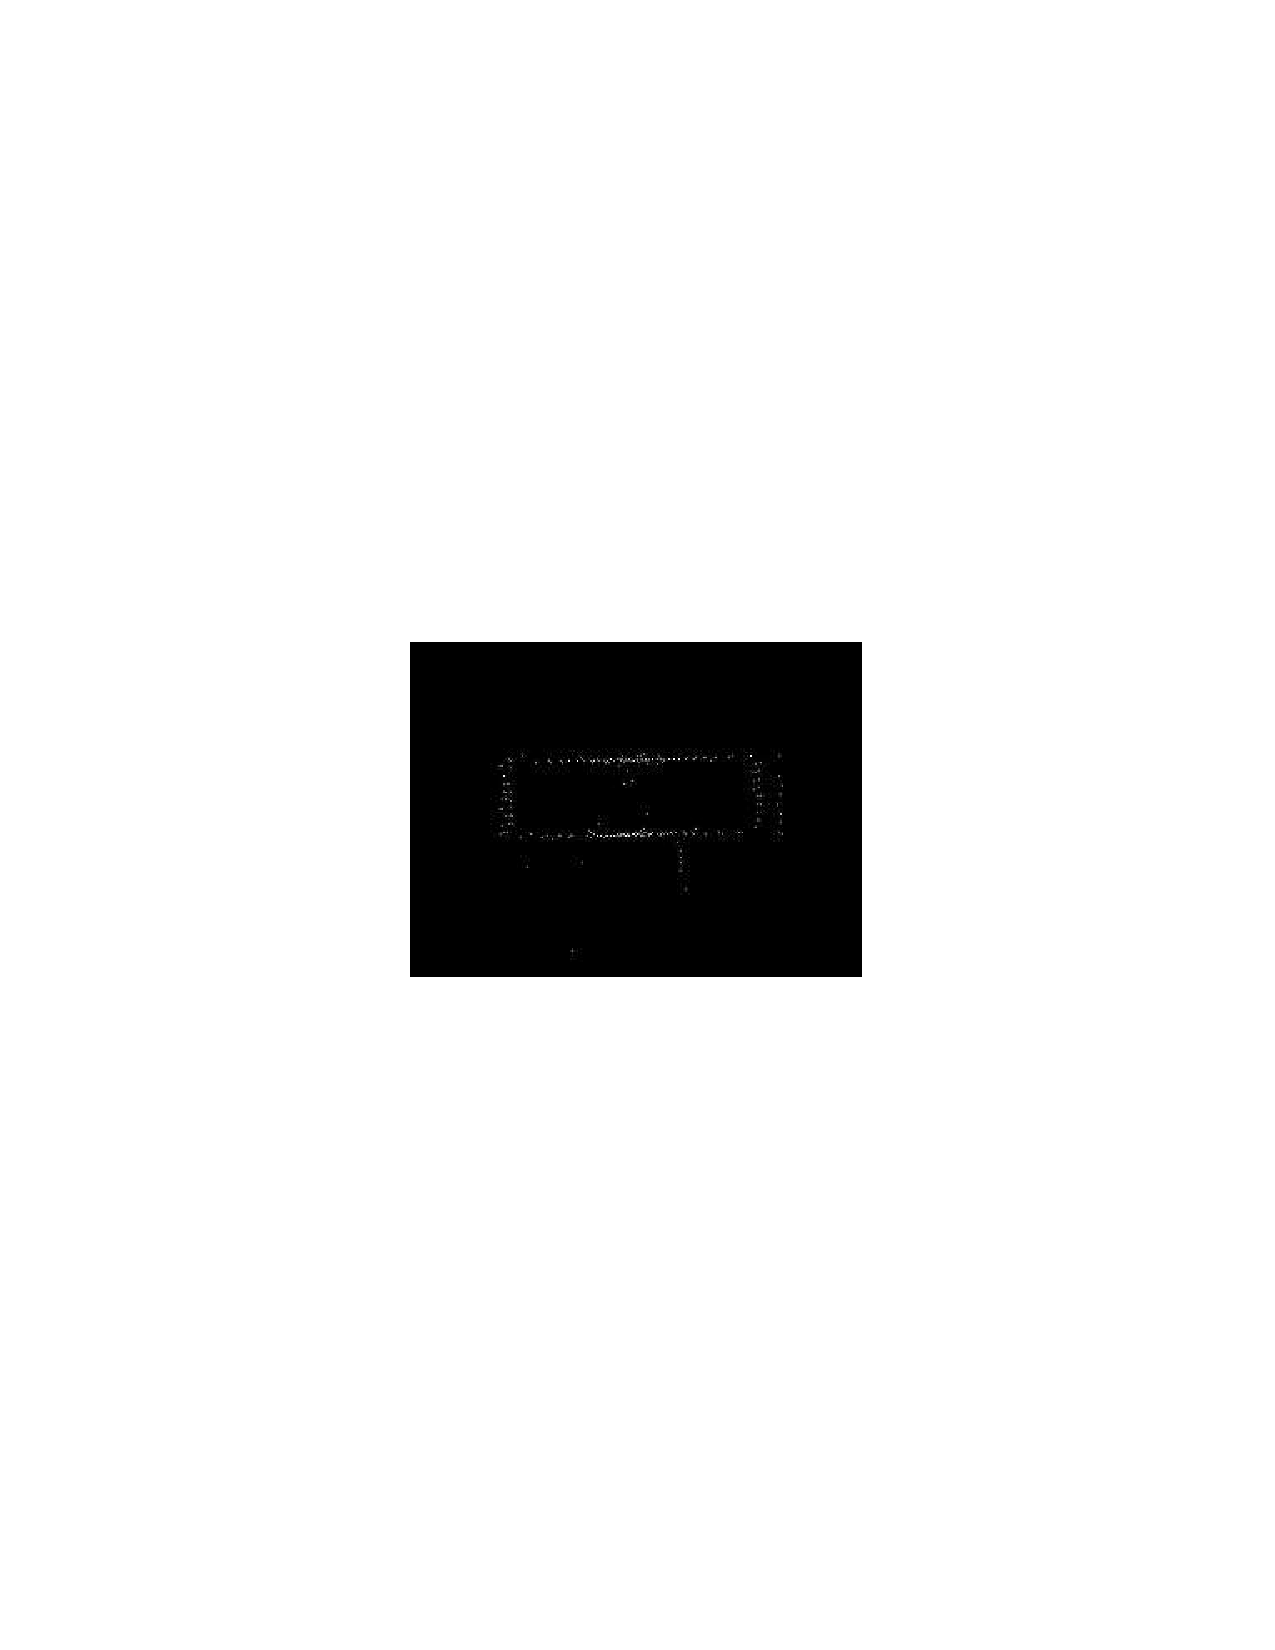
\includegraphics[scale=0.5]{flevoland_fusao_swt_crop.pdf}
	\caption{Fusão de evidências de bordas usando o método pca.}
\label{fig_07}
\end{figure}
\begin{figure}[hbt]
	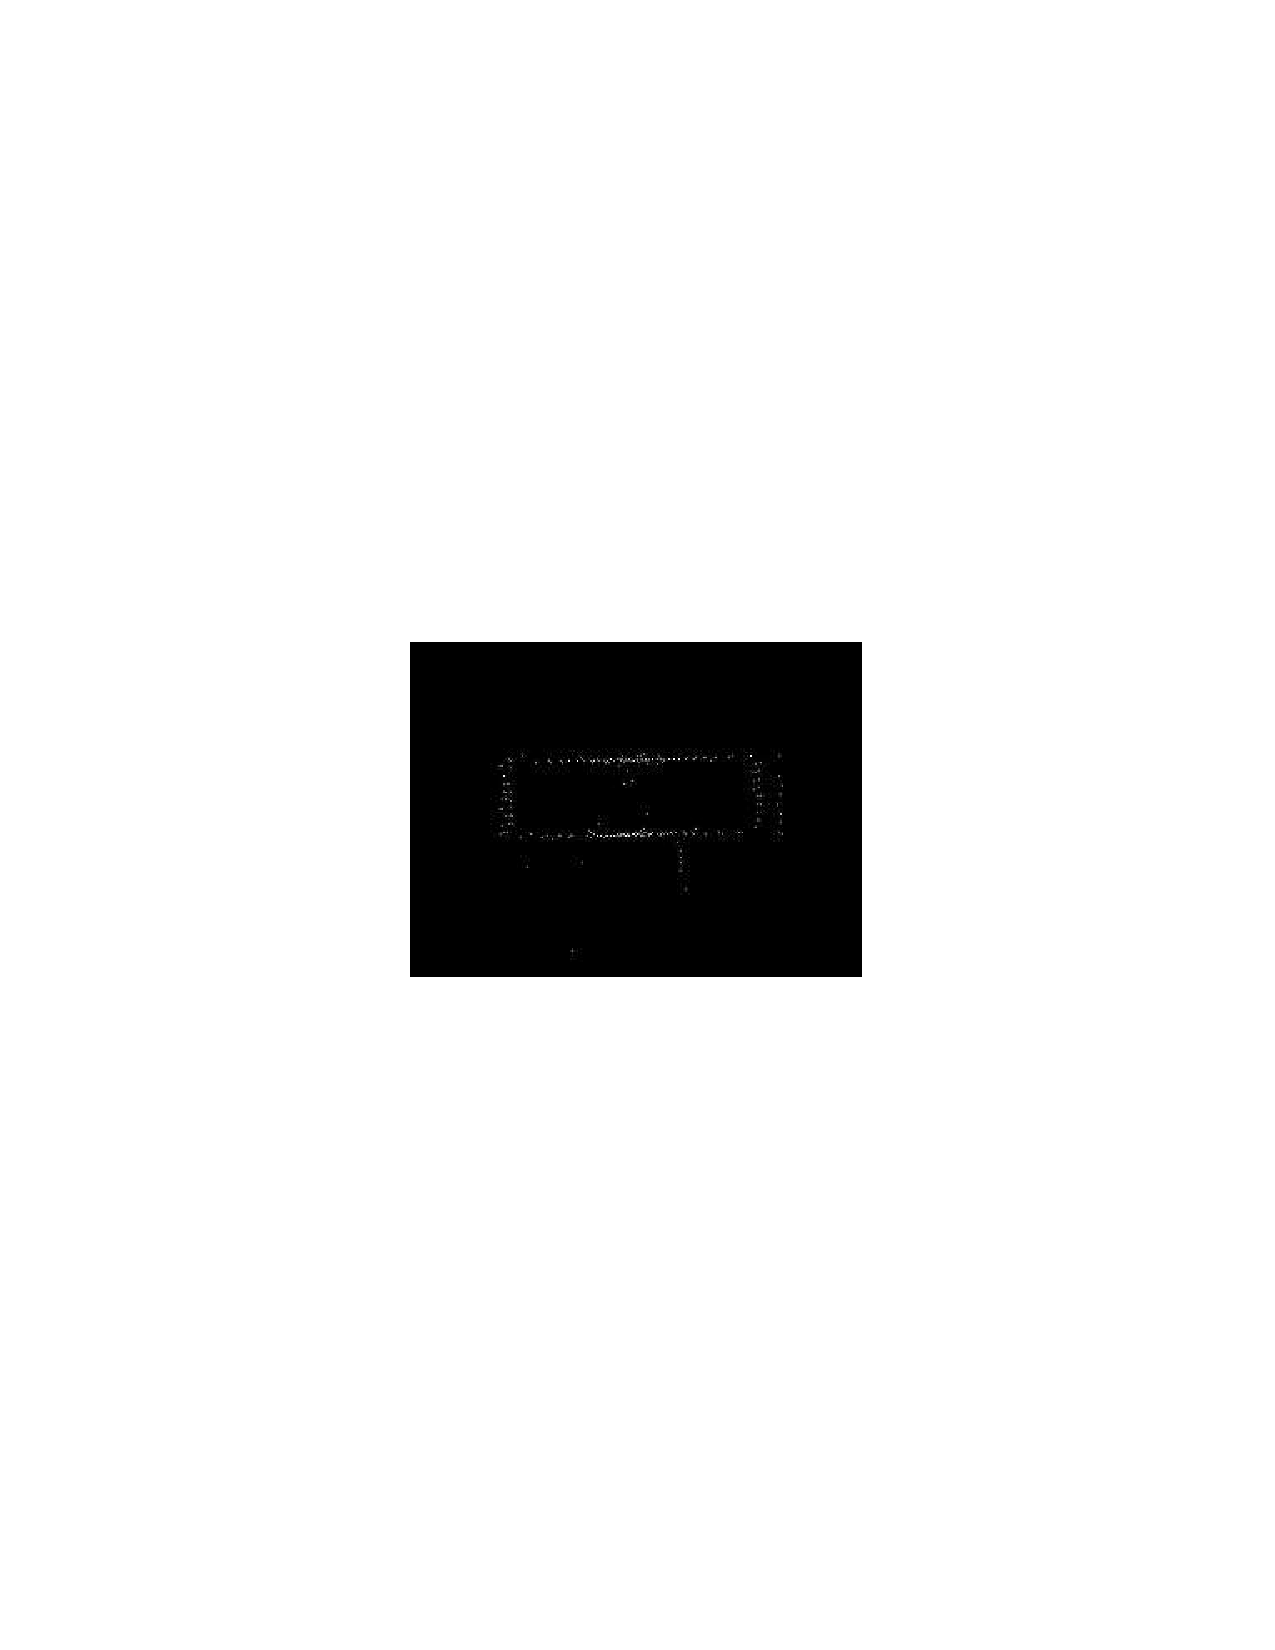
\includegraphics[scale=0.5]{flevoland_fusao_swt_crop.pdf}
	\caption{Fusão de evidências de bordas usando o método ROC.}
\label{fig_08}
\end{figure}

\section{Conclusão}\label{sec_08}
Nesse estudo, a abordagem de modelagem estatística foi aplicada em imagem de dados PolSAR real. Buscando-se entender a importância da informação de cada um desses canais na fusão de evidências de bordas. Foi aplicado o algoritmi proposto em três canais de intendidade (hh), (hv) e (vv). Inicialmente, encontramos as evidências de bordas, usando o método da máxima verosimilhança em cada um dos canais, obtendo-se bons resultados. Ao analisar os resultados obtidos nos três canais, observou-se que o método para a detecção de bordas funcionou bem nos canais (hh) e (hv) atingindo melhor acurácia em relação ao canal (vv).

Posteriormente, foi realizado a fusão de evidências de bordas com os métodos de média simples, SWT, PCA e estatística ROC. Os três primeiros métodos tiveram bom desempenho como mostram os resultados. O método de estatística ROC suprimiu vários pontos de bordas, comportamento esperado por ser um método que usa limiares, entretanto, ao ser aplicado em maior número de canais, seu desempenho tende a melhorar. 

Com base nesses resultados um possível caminho para melhorá-los seria aumentar o número de canais estudados. Abrindo espaço para futuras pesquisa aplicando-se outros métodos de fusão de evidências de bordas.

\bibliographystyle{IEEEtran}
\bibliography{bibliografia}
\end{document}
